\documentclass[a4page, 11pt]{article}

\usepackage{graphicx}
\usepackage{mathtools}
\usepackage[margin=0.65in]{geometry}
\usepackage[utf8]{inputenc}
\usepackage[english]{babel}
\usepackage[autostyle]{csquotes}
\usepackage{enumitem}
\usepackage[backend=biber]{biblatex}

\addbibresource{biblio.bib}


\graphicspath{ {./img/} }

\title{Data Management}
\author{}
\date{}
%NEED TO IMPROVE SECTION 6 DATA DISTRIBUTION
\begin{document}

\maketitle

%%% SOLO QUESTO E' ITALIANO %%%
\section{Data Modelling}
Il data modelling è uno strumento per descrivere parte del mondo reale che ci permette di:
\begin{itemize}[noitemsep]
\item Immagazzinare dati (write data)
\item Interrogare i dati (read data)
\end{itemize}
Un data model è composto prima di tutto da un modello concettuale (teoria) e poi da un linguaggio (anche grafico a volte) per descrivere e interrogare i dati. Un data model è sempre disponibile in un databasse management system che supporta la semantica del modello. Alcune delle caratteristiche più importanti di un data model sono:
\begin{itemize}[noitemsep]
\item Machine readability
\item Expressive power
\item Semplicità? Flessibilità? Standardizzazione?
\end{itemize}
Il data model più famoso  e conosciuto è il modello relazionale.
\subsection{Relational model}

Aspetti positivi :

\begin{enumerate}[noitemsep]
	 
	\item
	Molto rigido come regole.
	\item
	Il RDBMS sfrutta le proprietà ACID :
	\begin{itemize}
		
		\item
		A : Atomicity : serve affinché l'operazione o avviene su tutti i dati o non avviene, ad esempio se vi è un aggiornamento nei dati questo aiuta affinché i dati non vengano aggiornati solo parzialmente.
		\item
		C : Consistency : I dati o il nuovo dato che viene aggiunto rispetta lo schema prestabilito. E se si viola la consistenza con un'operazione tutta l'operazione fallisce.
		\item
		I : Isolation : gestisce come l'integrità delle transazioni sono viste dall'utente. Inoltre garantisce che durante un'operazione (query) non vengano svolte altre operazioni, e che lo stato del database venga modificato solo prima della fine della query.
		\item
		D : Durability : garantisce che una transazione effettuata sopravvivrà per sempre, anche se il sistema crasha. Dovuto grazie ai server di
		backup e log files.
	\end{itemize}
\end{enumerate}
Il RDBMS esiste già da 35 anni quindi è ben sviluppato e molto conosciuto, molti dati sono ancora salvati in questo formato ed è efficace ancora per molte operazioni. Gli aspetti limitanti sono:

\begin{enumerate}[noitemsep]
	 
	\item
	un attributo può avere solo un valore.
	\item
	non è compatibile con molti linguaggi moderni.
	\item
	molto rigido come linguaggio
	\item
	non accetta i loop.
	\item
	Per i RDBMS :
	\begin{itemize}
		
		\item
		Difficile modificare le tabelle.
		\item
		La performance.
	\end{itemize}
\end{enumerate}
Nei RDBMS la performance (inteso come velocità) dipende da vari fattori:
\begin{itemize}[noitemsep]
	 
	\item
	Numero delle righe
	\item
	Tipo di operazione
	\item
	Algoritmo scelto
	\item
	La struttura dati scelta
\end{itemize}
Per Scaling Up intendiamo potenziare le macchine, mentre per Scaling out intendiamo aggiungere macchine, per i RDBMS è più facile Scale up che Scale out. 
Il costo è un altro dei problemi, installare il software richiede un costo molto alto e hardware molto complesso.
Inoltre se continuiamo a aggiungere server (scaling out) il prezzo dell'Hardware aumenta esponenzialmente mentre il tempo di risposta scende asintoticamente.
\newline
\subsection{NoSQL}
Di fronte a questi svantaggi sorge una nuova ``tecnologia'' i NoSQL(Not Only SQL), le proprietà dei NoSQL sono:

\begin{enumerate}[noitemsep]
	 
	\item
	Non hanno nessuno schema o modello prefissato
	\begin{itemize}
		
		\item
		A differenza dei modelli SQL nei quali bisogna prima definire il modello, qua nei NoSQL non esiste un modello rigido.
		\item
		Per aggiungere un nuovo attributo non vi è bisogno di cambiare il modello a differenza dei SQL.
		\item
		I modelli NoSQL seguono l'assunzione del mondo aperto (ciò che non è vero è sconosciuto, ma non per forza falso) mentre SQL segue l'assunzione del mondo chiuso (solo ciò che è noto come vero è vero)
	\end{itemize}

	\def\labelenumi{\arabic{enumi}.}
	 
	\item
	Segue il teorema CAP:
	\begin{itemize}
		\item E' impossibile per un sistema informatico distribuito(vuol dire sistemi interconnessi tra loro e la comunicazione avviene solo attraverso messaggi) fornire simultaneamente le tre garanzie(infatti si possono soddisfare solo 2 di esse):
		\begin{enumerate}		
			\item
			\textbf{(C)C}onsistency(Coerenza) : Tutti i nodi vedono gli stessi dati allo stesso istante. Se è assente allora una soluzione è mostrare il dato precedente alla modifica cioè non quello più recente.
			\item
			\textbf{(A)}vailability(Disponibilità) : La garanzia che ogni richiesta ottenga una risposta su ciò che è fallito e ciò che ha avuto successo. Se è assente aspetterò per lunghi tempi senza ricevere una risposta.
			\item
			\textbf{(P)}artition Tolerance(Tolleranza sulle partizioni) : Il sistema funziona anche dopo aver perso un numero arbitrario di pezzi del sistema.
		\end{enumerate}
		\item
		I sistemi RDBMS sono dei software CA, ed è possibile creare dei modelli RDBMS basati sul CAP
		\item
		I sistemi NoSQL sono dei sistemi solitamente CP o AP.
		\item
		Uno preferisce la disponibilità sulla coerenza, perché è meglio vedere un vecchio dato non coerente che vedere un errore di fallimento di caricamento dei dati.
	\end{itemize}

	\item
	Segue Principio BASE:
	\begin{itemize}
		
		\item
		Basic Availability : completare una richiesta anche se parzialmente consistente, ad esempio nel caso di fallimento. E' possibile fare ciò grazie al fatto che usa server sparsi ovunque con un grado di	replicazione del database e in caso di malfunzionamento del database richiesto non tutto il sistema cede la disponibilità.
		\item
		Soft State : Abbandonano la richiesta di consistenza dei ACID praticamente completamente, cioè i dati possono avere schemi diversi.
		\item
		Eventual consistency : I sistemi NoSQL richiedono che a un certo punto i dati convergeranno a uno stato consistente (non si fa garanzie sul quando), e quindi prima di allora ho una consistenza ritardata cioè prima del momento dello stato consistente posso ricevere come risposta qualunque valore come risposta di una query.
	\end{itemize}
\end{enumerate}



\begin{center}
\begin{tabular}{|l|l|}
\hline
ACID & BASE \\
\hline
• Forte Coerenza & • Coerenza debole\\
• Poca disponibilità & • Disponibilità è la cosa principale\\
• Pessimo “Multitasking” & \quad e sacrifica per questo (CAP)\\
• Complesso & • Veloce e Semplice\\
\hline

\end{tabular}
\end{center}
Esempi e tipologie di modelli NoSQL :

\begin{enumerate}[noitemsep]
	 
	\item
	Key Value (Dynamo, Voldemort, Rhino DHT) : Sono delle tabelle con	chiavi che si riferiscono/puntano a un certo dato, è molto simile a Document based. 
	\item
	Column family (Big Table, Cassandra) : In grado di salvare grandi quantità di dati, la chiave colonna si riferisce a un certo dato ragruppato in colonna.
	\item
	Document based (CouchDB, MongoDB) : Di solito salvati con file JSON, salvati come una \textless{}chiave -- valore\textgreater{}. E' facile ricercare dati in questo formato. JSON è basato su due strutture :1) chiave -- valore per gli oggetti e 2) lista ordinata di elementi.
	\item
	Graph based (Neo4J, FlockDB) : Uso i vertici/nodi e archi per
	rappresentare i dati e legami tra di loro. E' difficile fare scaling	con i grafi per quanto riguarda l'immagazzinamento ma è molto rapido nelle query.
\end{enumerate}
Dobbiamo sacrificare o la dimensione del database o la sua non complessità:
\begin{center}
	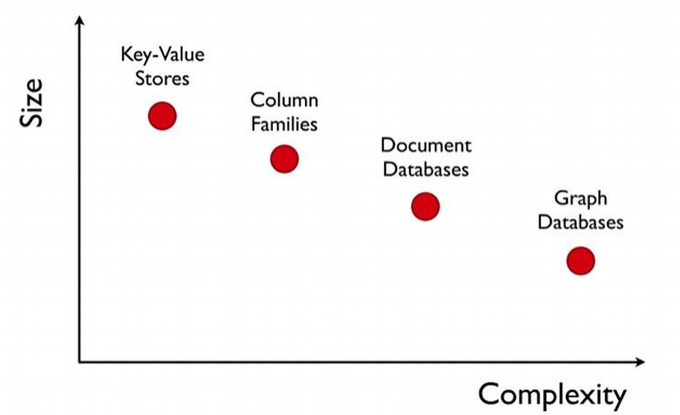
\includegraphics[scale=0.5]{IMAGE1.jpg}
\end{center}



\subsubsection{Document Based\cite{MongoDB}}
MongoDB is as already mentioned a document based management system, with the data stored in Bson (Binary Json), and the access to data is possible thanks to indexes. Compared to the SQL DBs, Mongo doesn't have the join feature. The name changes are:

\begin{center}
	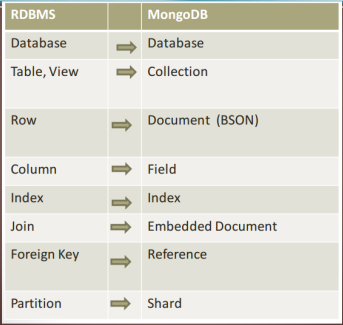
\includegraphics[scale=0.6]{IMAGE2.jpg}
\end{center}
In case of a massive data upload one might decide to do a few changes in the process to fasten  it up:

\begin{itemize}[noitemsep]
	 
	\item
	Disable the acknowledgment(ack) of the data, which is a signal passed between communicating processes, computers or devices, to signify acknowledgment or receipt of message, as part of a communications
	protocol.
	\item
	Disable the writing on a log file
\end{itemize}
One must be attentive when doing so because any loss will not be registered and lost forever.
\newline
For large data-sets it is useful to use some additional structures called indexes, they are similar to the book indexes and act as a faster way to retrieve information, they might require more time during the insertion but makes the queries faster later, one primary index (basic one) is always the defined for the id. How does it exactly works?
Basically without an index Mongo will perform a simple table scan (like SQL) in which it has to look through all the ``book'' to find a query result. The analogy with the book is if we don't have the index for our books we will have to read it whole until finding the point where we wanted to be. 
Indexing avoid this problem (more problematic if the database is large), it is an ordered list that points it's content.
Since indexing slows down the modifications one must choose just a couple of indexes for any given collection, the tricky part is to decide which one. MongoDB gives, by default, a limit of 64 indexes!
\newline
The aggregation uses pipeline and options. 
The aggregation pipeline starts processing the documents of the collection and passes the result to the next pipeline in order to get result for example: \$match and \$group. 
We can use the same operator in different pipelines.
\newline
Mongo for many reasons (mainly commercial) offers also a SQL interface; we need the connector BI (Business Intelligence): it generates the relational schema and use such schema to access the data.

\subsubsection{GraphDB\cite{Neo4J}}

A graph is a collection of nodes and edges which represents their relations. 
It has a lot of applications such as: social media, recommendations, geo, logistics network, financial transaction graphs (for fraud detection), master data management, bioinformatics, authorization and access control.
\newline
The labeled property graph model has the following characteristics:

\begin{itemize}[noitemsep]
	 
	\item
	It contains nodes and relationships;
	\item
	Nodes contains properties (key : value pairs);
	\item
	Nodes can be labeled with one or many labels;
	\item
	Relationships are named and directed, with a start and end node;
	\item
	Relationships can contain properties like nodes.
	\item
	%magari migliorare questa parte
	The relationship can be fine-grained or generic: for example in case of Address we can choose distinct relationship like HOME\_ADDRESS or WORK\_ADDRESS or DELIVERY\_ADDRESS which is the fine-grained relationship or we could choose only address and specify in it which kind of address it is ADDRESS\{type : `home'\} or the other ones. This method is called generic relationship. Usually the generic one is preferred,  especially in cases where I need to find all the address of a client: all I need to do is find the ADDRESS relationship, in the fine-grained I need to find one by one all kind of addresses, just	imagine if we had 100 types of addresses. On the other hand to find the DELIVERY\_ADDRESS all I need to do is find ADDRESS\{type:`delivery'\} 
\end{itemize}
A Graph Database (GD) can use either the native or non-native storage and processing engine.
\newline
Native Graph Storage is the one optimized for the native graph management \& the non native graph storage stores the data in non graph based model but this model supports a graph query language, examples: Relational, Object oriented DB, Wide Column. In a relational for example in a join bomb we can use a graph to connect two tables. But the problem
with the relational DBs and most of NoSQL DBs is that it lacks relationships.
Moreover in SQL joining tables adds more complexity, and in case of sparse table with null-able column require special checking in the code. In the case of a market, just to see what a customer bought, we need to do a lot of expensive joins on the customers that buy a specific product with other products for the recommendation systems. 
For the NoSQL DBs whether key-value, document or column-oriented, we might use the aggregation technique to see the relationship, but the relationship between aggregates aren't citizen in the data model and is costly operation since it doesn't use index free adjacency(the data is physically near) and since they stay inside of aggregates with structure in form of nested maps and even after the aggregation there is no back link to point backward and run
other interesting queries.
\newline
In a native graph storage the attributes and nodes and the referenced nodes are stored together, to optimize the graph processing engine. 
When we perform a query the graph model does not depend on the total number of nodes instead it remain nearly constant because it works locally to the portion of the graph which is connected to the base node, while the other SQL and NoSQL models will suffer in performance speed with the
increase of data. Moreover we can add more data/nodes and relationship without disturbing the already existing model.
\newline
The processing engine uses index-free adjacency, meaning that connected nodes physically points to each other in the DB, this makes sure that the retrieval is faster but it comes at a cost: the efficiency of queries that do not use graph traversal, for example the writing time etc.
\newline
It's important to note that it's neither good nor bad to use native or non-native engine, simply one needs to choose one based on his/her needs, for example my DB is based on a non-graph backend (like MySQL) so it would be useful to use a non native graph storage.
\newline
The properties of the cypher language is :

\begin{enumerate}[noitemsep]
	 
	\item
	Pattern-matching query language
	\item
	Humane language, easy to learn, read and understand
	\item
	Expressive yet compact
	\item
	Declarative : Say what you want, not how
	\item
	Borrows from well known query languages especially SQL, yet clearly it's different enough to see that it deals with graphs and not SQL	DBs.
	\item
	Aggregation, Ordering, Limit
	\item
	Update the Graph
\end{enumerate}
A real example is the following: We want to manage a server farm, we define a relational model for managing it. 
We know that a user access to application which runs on a VM and each application uses a DB and a secondary DB. 
Each of the VM is hosted on a server which are placed in a rack structure which is managed by a load balancer.
\newline
The initial stage of modeling is similar in any kind of DB, we seek to understand and agree on the entities in the domain and how to interrelate, usually done on whiteboard with a diagram which is a graph.
Next stage we seek a E-R (Entity-Relationship) diagram, which is another graph. 
After having a suitable logical model we map it into tables and relations. 
We keep our data in a relational DB, with it's rigid schema.
But keeping the data normalized slows down the query time so we need to denormalize it, because the user's data model must suit the database engine not the user. 
Denormalizing we involve duplicate data to gain query performance, denormalizing is not a trivial task and we accept that there may be substantial data redundancy. 
The problems doesn't stop here, because once created if we need to modify it, which we will need to do in order to match the changes in the production environment, so we will need to do this work all again!
\newline
It's better in there cases to directly use the graph DBs, it will avoid the data redundancy and it can adapt really fast in case of a change in the DB.
\newline
Another graph traversal language is Gremlin, part of the Apache TinkerPop framework. In this domain specific language (DSL) expressions specify a concatenation of traversal steps, so you basically explain to gremlin step by step what to do.

\subsubsection{Key-Value Model}

It's the most simple and flexible model of the NoSQL family, where every key is assigned to a value. It is possible to assign a type to a value.
The values are not query-able, such as a BLOB, where a BLOB(Binary Large OBject) is a collection of binary data stored as a single entity in a DB, for example images, videos etc.:
\begin{center}
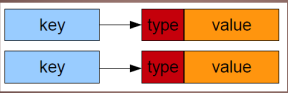
\includegraphics[scale=0.5]{IMAGE3.jpg}
\end{center}
An example is the amazon's cart system which uses DynamoDB, a key-value system.

~\\
The basic operation in a key-valued models are:

\begin{itemize}[noitemsep]
	\item
	Insert a new key-value pair
	\item
	Delete a new key-value pair
	\item
	Update a new key-value pair
	\item
	Find a value given the key
\end{itemize}
There is no schema and the values of the data is opaque. The values can be accessed only through the key, and stored values can be anything : numbers, string, JSON, XML, images, binaries etc.
An example of key-value model is Riak and has the following terminology:
%Quanto è figo minipage, l'ho scoperto dopo aver cercato come unire una tabella con un immagine xD!
\begin{center}
	\begin{minipage}[b]{0.4\textwidth}
	\begin{tabular}{|l|l|}
		\hline
		\textbf{Relational} & \textbf{Riak}\\ \hline
		database instance & Riak cluster\\ \hline
		table & bucket \\ \hline
		row & key-value\\ \hline
		rowid & key\\ \hline
	\end{tabular}
	\end{minipage}
	\begin{minipage}{.5\textwidth}\centering
	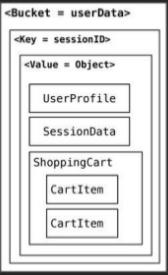
\includegraphics[scale=0.6]{IMAGE4.jpg}
	\end{minipage}

\end{center}
%Things not to remeber putting just for completation
Some other examples are: Redis, Memcached, Riak, Hazelcast, Encache.
\newline
Thanks to the Hash based index, the key-value systems can scale out in a very efficient way. 
The Hash is a mathematical function that assign to a given key it's value, usually we have h(x) = value, usually it returns a pointer to where the data is stored not exactly the data itself, for example h(x) = (x modulo y) where y is the max length of hash table. 
There might a problem with the conflicts but they can be managed. 
Hashing also enables items in the DB to be retrieved quickly. 
The hash table can be easily distributed in a network, it is managed in pile so we can have a key(saved in the pile) x saved in a server and it's succ(x) stored in a different server, thus scaling out really fast. 
The key value terminology is the following:
\newline
In a DHT(Distributed Hash Table) it is pretty simple to insert a key-value (k1,v1) basically take the key as input and route messages to the node holding that key and store the value there, and to retrieve the value of k1 it simply finds the node with the key k1 and return it's value v1 from it.

\subsubsection{Wide Column and BigTable}
These two models are an evolution, in a certain way, of the key-value models. When we start giving a structure to the value it becomes more complicated so we use wide column(Big Table): The first model was introduced by Google(HBase) and later on by Facebook (Cassandra) some think that Cassandra is still a key-value model and not a wide column.
\newline
BigTable is a multidimensional map, which can be accessed by row key, column key and a timestamp. It is sorted, persistent and sparse.
We will consider the \textbf{HBase BigTable} Model.
The data is organized in tables, each table(the tables are multi-versioned) is composed by the column-families that include columns, the cells within a column family are sorted physically and are usually very sparse with most of the cell having NULL value so we can have different rows with different sets of columns. 
BigTable is characterized by the row key, column key, timestamp, the row has the keys, column contains the data and contents. 
The column is divided in families. The timestamp support the multi-version of modification to check how the data changed over time and still be able to access the latest one without any confusion. We can represent it as follows:

\begin{center}
	\begin{tabular}{|c|c|c|}
		\hline
		\textbf{row key} & \textbf{column family 1} & \textbf{column family 2} \\
		\hline
		&
		\begin{tabular}{c|c}
			\textbf{column 1} & \textbf{column 2}
		\end{tabular}
		&
		\begin{tabular}{p{1.8cm}|p{1.8cm}|p{1.8cm}}
			\textbf{column 1} & \textbf{column 2} & \textbf{column 3}
		\end{tabular}
		\\
		\hline
		&
		\begin{tabular}{c|c}
		\textit{cell(data)} & \textit{cell(data)}
		\end{tabular}
		& 
		\begin{tabular}{p{1.8cm}|p{1.8cm}|p{1.8cm}}
		\textit{cell(data)}&\textit{cell(data)} &\textit{cell(data)}
		\end{tabular}\\
		\hline
		&
		\begin{tabular}{c|c}
			\textit{cell(data)} & \textit{cell(data)}
		\end{tabular}
		& 
		\begin{tabular}{p{1.8cm}|p{1.8cm}|p{1.8cm}}
			\textit{cell(data)}&\textit{cell(data)} &\textit{cell(data)}
		\end{tabular}\\
		\hline
	\end{tabular}\\
	~\\
	Each row can have different timestamp, so we can have more versions of this table.
\end{center}
The data within the cells (also the key) is without type since it is saved in bytes. The columns are dynamic. So to get a data given a key we need to transform our data in Bytes with a comand .toBytes(``Key''), we can also use python to modify the columns via APIs. This model can be useful for *-To-Many mappings.
The row key is an array of bytes and serves as a primary key for the table.
Each Column Family has a name and contains one or more related columns, the columns can belong to one column family only and is included inside the row with familyName:columnName followed the value, for example we have: \\ 
%cavolo che sbatti i quote i LaTeX, se trovate un modo carino ditemelo
row key $|$ info:\{`height':`170cm', `state':`NY'\}  roles:\{`ASF':`Director', `Hadoop':`Founder'\}$|$\\
The version number of each row is unique within the row key, by default it uses the system's timestamp but they can be user supplied.
\newline
Best time to use HBase is when one need to scale out, need random write and/or read, when we need to do thousand of operations per second on multiple TB of Data, when we need to know all the modification done on
the data, when we need a well known and simple access. One can combine a GraphDB with HBase, one example is JanusGraph.
HBase does not support joins, but this can be done in application layer using Scan() and Get() operations of HBase.
\newline
\newline
\textbf{Cassandra\cite{Facebook}}: It started as a support for the Facebook inbox search, it was open sourced in 2008 by Facebook and then it became a top-level project under Apache in 2010. The data model is the same as HBase, the only difference is the way it is stored (storage model) and the program algorithms. We can say it is a restricted BigTable, we can have only one column family. It uses a C* language very similar to SQL language.
\newline
Cassandra is a column oriented NoSQL system. 
The KeySpace is the outermost container, it's basic attributes are the Replication Factor (how many copies of the data we need), Replication Strategy and the Column Families.
The Column Families, can be seen as a collection of rows or better a collection of key-value pairs as rows. 
A row is a collection of columns labeled with a name, the value of a row is itself a sequence of key-value pairs where the keys are the column's name and we need at least one column in a row. The columns have the key(name), the value and the timestamp. So a table is a list of “nested key-value pairs”: (ROW x COLUMN key x COLUMN value) and this is inside a column family.
The Key Space is only a logical grouping of columns families.

\begin{center}
	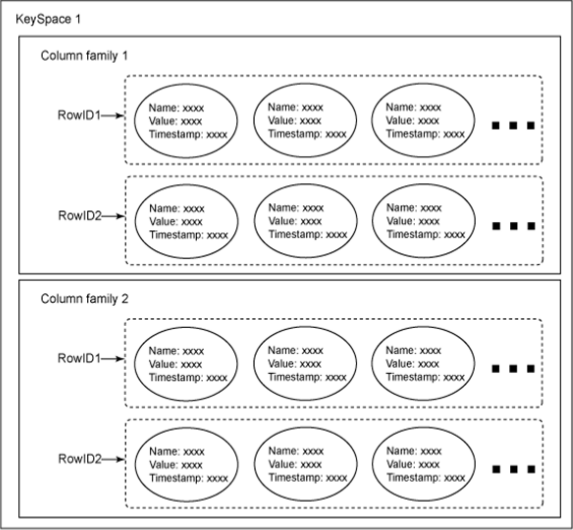
\includegraphics[scale=0.5]{IMAGE5.png}\\
	An example of Cassandra data model.
\end{center}
While with RDBMS, we can have that JOIN of normalized tables can return almost anything, with C* the data model is designed for specific queries and the schema is adjusted as new queries are introduced. In C* there are no JOINS, relationship or foreign keys and the data required by multiple tables are denormalized across those tables.
\newline
The Comparison between Apache Cassandra, Google Big Table and Amazon DynamoDB is:
\begin{center}
	\begin{tabular}{|p{3.6cm}|p{3.6cm}|p{3.3cm}|p{4cm}|}
		\hline
		&\textbf{Apache Cassandra} & \textbf{Google Big Table} & \textbf{Amazon DynamoDB}\\
		\hline
		\textit{Storage Type} & Column & Column & Key-Value\\
		\hline
		\textit{Best Use} & Write often\newline read less & Designed for\newline large scalability & Large database solution\\
		\hline
		\textit{Concurrency Control} & MVCC & Locks & ACID\\
		\hline
		\textit{Characteristics} & High Availability\newline Partition\newline Tolerance\newline Persistence & Consistency \newline High Availability\newline Partition\newline Tolerance \newline Persistence & Consistency \newline High Availability\\
		\hline
	\end{tabular}
\end{center}

\section{Data Distribution}
\subsection{Fragmentation and Replication}
A centralized DB system is a system where the database is located, stored and maintained in a single location. If the processor fail all the system fails.
If we need data periodically in different location we can distribute it or replicate it. The distribution is to divide the data and have it stored in different places, it provides opportunities for parallel execution. On the other hand we can also replicate it or replicate part of data in different location improving also the availability.
\newline
In a Homogeneous Distributed Database all sites have identical software and aware of each other and agree to cooperate in processing user requests. They surrender their autonomy to change the schema appearing to user as a single system.
\newline
In a Heterogeneous Distributed Database different sites may use different schema and software which creates a major problem for query and transaction processing. The sites may not be aware of each other and may provide only limited facilities for cooperation in transaction processing.
\newline
The challenges of a distributed database design is deciding what goes, which depends on the data access pattern, and the problem of where to allocate fragments to nodes.
With replication we have that system maintains multiple copies of data, stored in different sites, for faster retrieval and fault tolerance and with the fragmentation the data is divided into several fragments stored in different sites. We can combine both of them so the data is partitioned into several fragments and the system maintains several identical replicas of such fragment.
\newline
Dividing/fragmenting our database into n databases, the bottom-lake phenomena arises, in which the slowest machine becomes the bottom-lake: the maximum time for a query is dependent on that machine.
\newline
The advantages of replication are:
\begin{itemize}[noitemsep]
	\item
	Availability: Since the failure of a site does not result in unavailability of it's data since it's replicas exist elsewhere.
	\item
	Parallelism: Queries may be processed by several nodes in parallel thus faster.
	\item
	Reduced data transfer: Since replicas of the data may exist in the node itself.
\end{itemize}

While the disadvantages are:

\begin{itemize}[noitemsep]
	 
	\item
	increased cost of updates: Since each replica must be updated.
	\item
	increased complexity of concurrency control e.g. two people book a ticket at the same time solution. We may have that distinct replicas may lead to inconsistent data unless some special concurrency mechanisms are implemented. A solution could be to choose one copy as the primary copy and apply concurrency control operation only on the primary copy.
\end{itemize}
As already mentioned we can combine data replication with data fragmentation. In particular data fragmentation consists in a division of relation r into fragments which contain sufficient information to reconstruct relation r.
Now for simplicity imagine the database to be relational. 
The fragmentation can be horizontal or vertical, but it must contain sufficient information to reconstruct the original "relation". In the horizontal each tuple of the data is assigned to one or more fragments while in the vertical the schema (in the case of relational) is split into several smaller schemas, and all of them must contain a common candidate key to ensure lossless join for example using a tuple-id attribute.\newline
The advantages are:
\begin{itemize}[noitemsep]
	\item Horizontal:
	\begin{itemize}[noitemsep]
		\item Allows parallel processing on fragments.
		\item Allows the data to be split so the tuples are located where they are more frequently accessed.
	\end{itemize}
	\item Vertical
	\begin{itemize}[noitemsep]
		\item Allows tuples to be split so that each part of tuples are stored where they are more accessed.
		\item tuple-id allows efficient joining of vertical fragments.
		\item Allows parallel processing on a relation.
	\end{itemize}
\end{itemize}
The two fragmentation can be mixed together and the fragments may be successively fragmented to an arbitrary depth. 
Data Transparency is very important because it indicates the degree to which the users are not aware on the way the data is stored in a  distributed system. 
We have to consider transparency issues in relation to: fragmentation, replication and location of our data.
\newline
Considering the difference between the centralized and the distributed system from the point of view of costs we have that:
\begin{itemize}[noitemsep]
\item For centralized systems, the primary criterion for measuring the cost of a particular strategy is the number of disk accesses.
\item In a distributed system, instead, other issues must be taken into account: in first place we have to consider the cost of a data transmission over the network and then also the potential gain in performance from having several sites process parts of the query in parallel.
\end{itemize}
Summarizing we have that the advantages of DDBMSs are: It reflects the organizational structure, improves share-ability and local autonomy, improves availability, reliability and performance, reduces the hardware cost and have a modular growth.
The disadvantages are: Architecture and database design is more complex, cost, Security, Integrity control is more difficult, there is a lack of standards and experience.
\newline
There are 3 types of architecture in DDBMS:
\begin{itemize}
\item Shared Everything: Dominated the architecture market until 2000(approximately), we have one big complex costly data base, it shares everything and can be very slow. It is the centralized system.

\item Share Disk: We have data saved on different disks connected between them, no one uses it. The disks are all connected together and communicates to all the CPUs.

\item Share Nothing: Every thing is separated every disk has it's own CPU and the disks does not communicate with other CPUs or disks, it is very easy to scale it out. Model adopted by NoSQL models. Only at the end the processors are connected together to combine the results from each of them. 
\end{itemize}

\begin{center}
	\begin{tabular}{|c|c|}
		\hline
		\textbf{Shared Disk} & \textbf{Shared Nothing}\\
		\hline
		Quick adaptability to changing workloads & Can exploit simpler, cheaper hardware\\
		\hline
		High availability & Almost unlimited scalability\\
		\hline
		Performs best in a heavy read environment & Works well in high-volume, read/write environment\\
		\hline
		Data need not to be partitioned & Data is partitioned across the cluster\\
		\hline
	\end{tabular}
\end{center}
What to choose between Scalability or Availability? It depends on how much one wants to spend: more availability means more money. For example a 100\% availability mean no downtime, decreasing the availability increases the downtime we can have, a 99\% availability means a downtime of 9 - 88 hours.
\newline
\textbf{Replication}:
\newline
A log is a sequential file that is stored in a stable(never failing) memory, it stores all activities realized by all transaction in a chronological order. The two types of records are the transaction logs (operations) and the system events (Checkpoint \& Dump). About this we can define checkpoint as the moment when we store the set of running transactions in a given time point while a dump is full copy of the entire state of a DB in a stable memory, his execution is offline and, summarizing, it generates a backup. Only after the backup is completed, the dump record of log is written.
\newline
The replicas structures are:
\begin{itemize}[noitemsep]
	\item One2Many: One source and many targets.
	\item Many2One: Many sources and only one target.
	\item Peer2Peer: Data is replicated across multiple nodes that communicates with each other.
	\item Bi-directional: Conceptually a Peer2Peer with only two Peers.
	\item Multi-Tier Staging: The replication is divided in more stages.
\end{itemize}

To create a replica we can:
\begin{itemize}[noitemsep]
	\item take the data form master either the backup copy or the data itself	(if we can stop the activity of the server) and move it. (It could be useful if the data is not accessible from outside)
	\item use log file : to maintain the replica the same as the source even during the transfer (near real time) using the Log to execute the same commands executed on the source.
\end{itemize}


%If you use Volume in project be attentive to the scalability!!!!!
\subsection{MongoDB's Approach: Sharding\cite{ScalingMongoDB}}

MongoDB uses Sharding to split a large collection across several servers(called a cluster): Every document has a key in mongodb so we define a shard key which defines the range of data(chunk range). The key space is like points on a line and the range is a segment of that line.
Example: Key is surname so we can decide all the surnames staring from A to K save in first partition and the others in the second.
MongoDB does the sharding automatically once we tell it to distribute the data. 
The Default maximum chunk size is 64Mb, as a chunks gets bigger, MongoDB will automatically split it into two smaller chunks and if the shards become unbalanced, some chunks will be migrated to other shards with less chunks correcting the imbalance. 
The goal of balancer is not only to keep the data evenly distributed but also to minimize the amount of data transferred. 
The balancer is lazy so it won't activate itself until the data is very imbalanced, it does so to avoid moving data back and forth, if it balanced every tiny difference it would just waste resources.
\newline
When you first create a shard, MongoDB creates a single chunk with range $(-\infty, +\infty)$ where with $-(+)\infty$ we mean the smallest(largest) value MongoDB can represent. 
From here if the chunk size is bigger that the chosen size it will split and every chunk range must be distinct and not overlapping and their union should cover all the initial range.
\newline
The shard is basically a server so we need to use mongos (s=server) to make a query on a shard. Mongos is the point interaction between users and the cluster, mongos lets you treat a cluster as a single server. 
The queries are routed to the appropriate shard thanks to mongos. For the not targeted queries (with sorting) a request is sent to all shards and the queries are performed locally and then after the result has returned mongos merges the (sorted) result and returns results to client.
Mongos doesn't actually store any data, the configuration of a cluster is held on a special mongods called config servers, they hold the definitive information about the clusters for everyone's access.
\newline
The cluster consists basically of three types of processes:
\begin{itemize}[noitemsep]
	\item The shards: a node of the cluster, it can be either a single mongod or a replica set. 
	MongoDB also automatically replicates the data and in one shard I will have a primary chunk where I store the data I wanted and secondary chunks where MongoDB replicated other data as backup just in case, the secondary is a read only data so I cannot do update queries on it.
	\item Mongos processes: for routing requesting to the correct data and acting as a balancer. It contains no local data and we can have 1 or many of it. After it finishes balancing it must also update the Config Servers with the new positions and while one mongos is balancing the chunks it takes out a "balancer lock" so no other mongos will start the balancing. The lock is released only after the chunk has been copied and the old chunk is deleted from the initial shard.
	\item Config servers: for keeping tracks of the cluster's state. It stores the cluster chunk ranges and locations.
	We can have only 1 or 3.
\end{itemize}

\begin{center}
	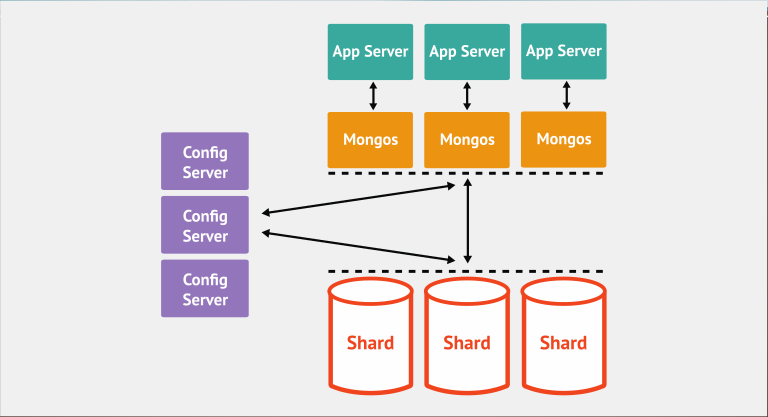
\includegraphics[scale=0.50]{IMAGE6.png}
\end{center}


Let's see the steps for the configuration:

\begin{enumerate}[noitemsep]
	\item Start a config server, it start by default at port 27019:

	mongod --configsvr
	\item Start the mongos Router, we need to initialize it like this even if the cluster is already running:
	
	For 1 configuration server: 
	mongos --configdb $<$hostname$>$:27019
	
	For 3 configuration servers:
	mongos --configdb $<$host1$>$:$<$port1$>$,$<$host2$>$:$<$port2$>$,$<$host3$>$:$<$port3$>$
	
	We can have different mongos on same pc on different ports.
	\item Start the shard database, it starts a mongod with the default shard port 27018
	
	mongod --shardsvr
	
	The shard is not yes connected to the rest of the cluster and it may have been already running in production.
	\item Add the Shard:
	
	On mongos: 
	sh.addShard('$<$host$>$:27018')
	
	To add a replica set: 
	sh.addShard('$<$rsname$>$/$<$seedlist$>$')
	\item Verify that the shard was added:
	
	db.runCommand(\{ listshards:1 \}) \newline
	Obtaining as result: \newline
	\{\newline
	"shards": \newline
	[\{ "\_id":"shard0000", "host":"$<$hostname$>$:27018"\}], \newline
	"ok" : 1 \newline
	\}
\end{enumerate} 
To enable sharding on a database simply use the command: sh.enableSharding("$<$dbname$>$") 
\newline To start a collection with the given key:
sh.shardCollection("$<$dbname$>.$people",\{"country" : 1\})
\newline
The properties of the Shard key are:
\begin{itemize}[noitemsep]
	\item Shard key is immutable
	\item Shard key values are immutable
	\item Shard key must be indexed
	\item Shard key are limited to 512 bytes in size
	\item Shard key are used to route queries: so choose a field commonly used in queries for the shard key
	\item Only the shard key can be unique across shards, the `\_id' field is only unique within the individual shard
\end{itemize}

\subsection{HBase}
The four major components (nodes) of HBase are:
\begin{enumerate}[noitemsep]
	\item The HMaster (only one): It is the implementation of Master server in HBase architecture. It monitors and coordinates all slaves in the cluster. It must assign regions, detect failures and has admin privileges. 
	\item The HRegionServer (many of them): It manages the data regions and serves client requests for reads and writes (using a log), this request is assigned to a specific region, where actual column family resides. However the client can contact directly the HRegionServer without having a permission of HMaster. HMaster is required only for operations related to metadata and schema changes. The Region servers run on Data Nodes present in the Hadoop cluster.\newline
	The HRegions are the basic building elements of HBase cluster that consists of the distribution of tables, i.e., a subset of a table's rows, like horizontal range partitioning and it is done automatically.
	\item The HBase client
	\item Zookeeper: It is a centralized monitoring server which maintains configuration information and provides distributed synchronization between nodes.
	HBase lives and depends on ZooKeeper, by default HBase manages the ZooKeeper instance (start and stop). 
	HMaster and HRegionServers register themselves with ZooKeeper.
	If the client wants to communicate with regions, the servers client has to approach ZooKeeper first.
	During a failure of nodes ZooKeeper Quoram will trigger error messages, and it starts to repair the failed nodes.
\end{enumerate}
HBase's architecture is similar to MongoDB's and they share the same flaw: If the master is broken the client cannot obtain any data and we have an error (Single point of failure).

\subsection{Cassandra}
Cassandra on the other hand repairs the flaw of having a single master because there is no master and all the nodes are considered the same, it uses a peer-to-peer distributed system. 
The Data is partitioned among all nodes in the cluster and a custom data replication to ensure fault tolerance and since all the nodes are all considered same we have Read/Write-anywhere design.
Cassandra is based on Google BigTable and Amazon Dynamo so it inherits their properties.
\newline
In Cassandra we can add or remove nodes with no downtime so we have a transparent elasticity and transparent scalability (performance grows linearly with the number of nodes) and due to it's P2P architecture we obtain also the High Availability. If a node were to fault we will have that we could obtain the data from the replicas in the other nodes.
The Nodes are logically structured in Ring Topology, the hashed value of key associated with data partition is used to assign it to a node in the ring. The hashing rounds off after a certain value to support the ring structure and the lightly loaded nodes moves position to alleviate the highly loaded nodes.
Cassandra uses ZooKeeper to find the replicas in other nodes, given a node we decide the N number of following nodes in which the replica will be saved.
\newline
The data writing is separated in 3 stages : 
\begin{enumerate}
	\item The log file writing, which is essential: even if the data writing fails it doesn't matter because we have the log file.
	\item Once written in the commit log, data is written to the mem-table. Data written in the mem-table on each write request also writes in commit log separately. Mem-table is a temporary storage of data in the memory while commit log logs the transaction records for backup.
	\newline The first place where the read operations take place is mem-table and several may exist at once (1 current and other waiting to be flushed). 
	\item When mem-table is full, flush the data from the mem-table and store them disk in SSTables. The SSTables are immutable once written.
\end{enumerate}
The consistency can be based on majority: if a certain number,which we decide(it can also be one), of the nodes agree that a certain data was written or read it is assumed to be true; \newline
or it can be based on quorum which states the $50\%\text{(of the replication factor)}+1$ nodes agree that something is written it's assumed true.
\newline
The commands for writing for write consistency one(quorum): \newline
INSERT INTO table (column1, ...) VALUES (value1, ...) USING CONSISTENCY ONE (QUORUM)\newline
If a node is offline, an online node makes a note to carry out the write once the node comes back online.
For reading the data we have the following command:
SELECT * FROM table USING CONSISTENCY ONE
\newline
To delete the data is it easier to consider the data not available and mark it for deletion, it is called a tombstone(like how recycle bin works in OS), and actually delete on a major compaction or configurable timer.\newline
Compaction runs periodically to merge multiple SSTables reclaiming space, creating new index, merging the keys, combining columns and discarding the tombstones.
%Sezione in italiano ricavata dagli appunti dell'anno scorso.
%Per ora non si sa se questa parte sarà richiesta all'esame.
%Da integrare se disponete di appunti affidabil ricavati a lezione
\section{Big Data Architecture}
La prima definizione di "Big Data" viene data da Gartner nel 2012: “Big data is high volume, high velocity and/or high variety information assets”. Ad oggi sappiamo però che per definire i "Big Data" potremmo usare più di 3 V, aggiungendo anche variability e veridicity. Analizzare "Big Data" su un singolo server “big” è un processo lento, costoso e difficile da realizzare. La soluzione è effettuare un’analisi distribuita su hardware poco costosi tramite un sistema di calcolo parallelo, i cui vantaggi sono già stati esposti nella sezione dedicata all'architettura distribuita. I problemi principali della distribuzione dei dati sono la sincronizzazione, i cosiddetti “punti morti” (deadlock), la larghezza della banda, la coordinazione tra i nodi e i casi di fallimento (failure) del sistema. Questo genere di architettura ha comunque molti vantaggi, tra cui: scala linearmente (scale out), l’attività di calcolo è rivolta ai dati e non viceversa (cambio di paradigma), gestisce i casi di fallimento (failure) e lavora con hardware con potenza di calcolo “normale”.
\subsection{HDFS}
L’architettura HDFS (Hadoop Distributed File System) è un file system distribuito progettato per girare su hardware base (commodity hardware).
\begin{center}
	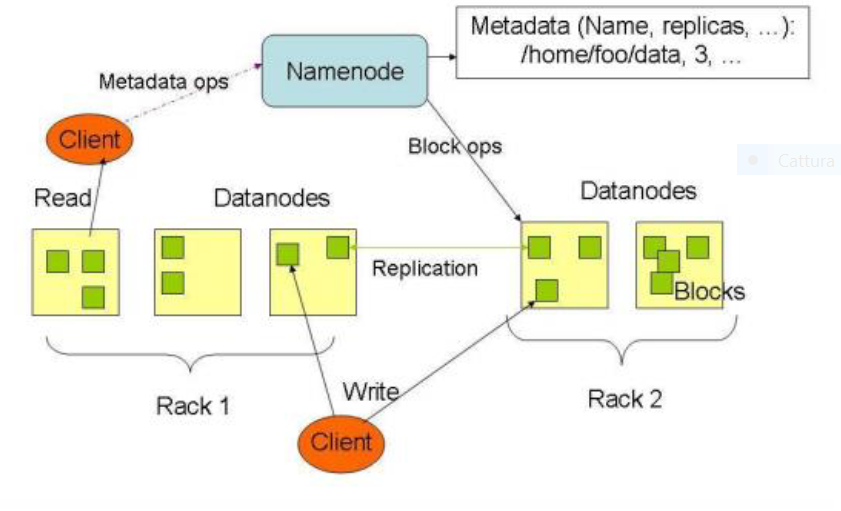
\includegraphics[scale=0.70]{IMAGE7.png}\\
	HDFS Architecture
\end{center}
Sebbene ci siano molte similitudini con altri sistemi di file system distribuiti, le differenze sono comunque significative. In particolare, HDFS è fortemente tollerante agli errori
ed è progettato per girare su macchine poco costose, inoltre fornisce un accesso ad alta velocità ai dati delle applicazioni ed è ideale per applicazioni con data set di grandi dimensioni. HDFS ha un’architettura master/slave. Un cluster HDFS consiste in un singolo NameNode e in un server master che gestisce il file system detto NameSpace e che regola gli accessi ai file da parte dei clients. Inoltre, sono presenti un certo numero di DataNodes, generalmente uno per ogni nodo nel cluster, che gestiscono lo storage collegato ai nodi su cui vengono eseguiti. Internamente, un file è splittato in uno o più blocchi (tipicamente di 128 MB ciascuno) e questi sono memorizzati in un set di DataNodes. Il NameNode esegue le operazioni del file system NameSpace, ovvero apertura, chiusura e “rename” dei file e delle directories. Inoltre, determina la mappatura dei blocchi nei DataNodes. I DataNodes sono responsabili invece delle richieste di operazioni di lettura e scrittura da parte del file system dei clients. I DataNodes permettono anche la creazione, l’eliminzazione e la replica dei blocchi sotto istruzioni del NameNode. I Meta-Data (lista dei file, lista dei blocchi, lista dei DataNodes, attributi del file, …) sono tutti memorizzati nella memoria principale. Esiste inoltre un Transaction Log che registra la creazione, l’eliminazione e qualunque altra operazione avvenga su un file.
La strategia di piazzamento dei blocchi del file tra i DataNodes è la seguente:
\begin{itemize}[noitemsep]
\item Una replica sul nodo locale
\item Una seconda replica su un rack (collezione di nodi) remoto
\item Una terza replica sullo stesso rack remoto
\item Delle repliche piazzate in modo randomico
\end{itemize}
I client leggeranno il file dalla replica più vicina a loro (rack awareness). Esiste poi un sistema per verificare la correttezza dei dati. Può succedere infatti che un blocco inviato dal DataNode arrivi corrotto. Il client software HDFS implementa un controllo checksum dei file. Quando un utente crea un file, genera anche un checksum per ogni blocco del file e memorizza questi checksum in un file nascosto separato nello stesso NameSpace HDFS. Quando un client richiede l’accesso al file, verifica che i dati ricevuti da ogni DataNode combacino con il checksum associato. Se così non è, il client deciderà di reperire quel determinano blocco da un altro DataNode che possiede una replica di tale blocco di dati. Il NameNode verifica inoltre che i DataNodes, i quali inviano continuamente “segnali di vita”, siano tutti funzionanti e gestisce gli eventuali malfunzionamenti. Tuttavia, il NameNode rappresenta un “single point of failure”. Per questo motivo i Transaction Log sono memorizzati in più directrories: nel file system locale e in uno remoto.\newline
Formati di file supportati: Text, CSV, JSON, SequenceFile, binary key/value pair format, Avro*, Parquet*, ORC, optimized row columnar format.
\subsection{Map Reduce}
Map Reduce è un motore di computazione distribuito. Ogni programma è scritto in uno stile funzionale ed è eseguito in parallelo. “Mapred” risolve problemi legati a Map Reduce quali:
\begin{itemize}[noitemsep]
\item Come assegnare i 'lavori' ai singoli 'worker'
\item Cosa succede se ci sono più 'lavori' che 'worker'
\item Cosa succede se i 'worker' devono condividere risultati parziali
\item Come aggregare i risultati parziali
\item Come scoprire se tutti i 'worker' hanno finito il proprio task
\item Cosa succede se un 'worker' muore
\end{itemize}
\begin{center}
	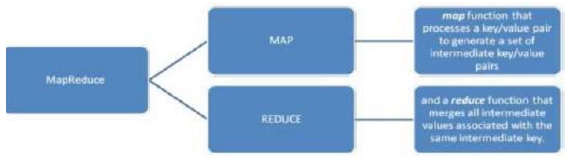
\includegraphics[scale=1]{IMAGE8.png}\\
	Map Reduce
\end{center}
La fase di Map esegue lo stesso codice su un grande ammontare di record, estrae le informazioni rilevanti, le ordina e le unisce. La fase di Reduce aggrega i risultati intermedi e genera l’output. Il programmatore dovrà esclusivamente definire le due funzioni di map e di reduce. Tutte le altre attività le svolge il mapred.
\subsection{Hadoop}
Hadoop è un framework che supporta applicazioni distribuite con elevato accesso ai dati, unisce il sistema MapReduce (parallel and distributed computation) e l’HDFS (hadoop storage and file system).
\begin{center}
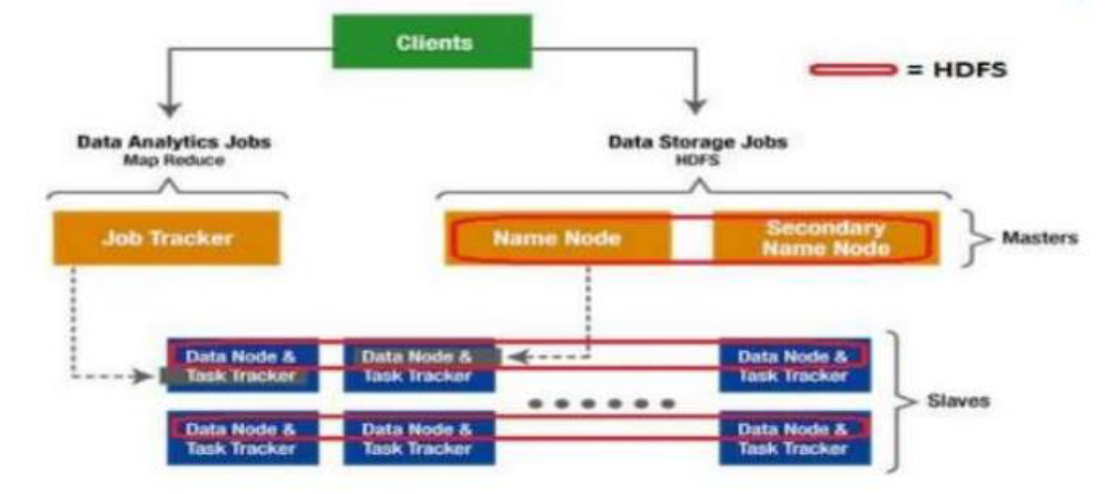
\includegraphics[scale=0.70]{IMAGE9.png}\\
Schema ecosistema Hadoop
\end{center}
Pig è uno scripting language che esegue l’analisi dei dati. Gli script in “pig latin” sono tradotti in lavori di MapRed. Hive è un’interfaccia simile a SQL per dati memorizzati in HDFS. I piani di esecuzione sono generati automaticamente da Hive. Hive rappresenta quindi un data warehousing basato su Hadoop. Questo applicativo è utilizzato per report giornalieri, misure di attività degli utenti, data e text mining, machine learning e per attività di business intelligence come pubblicità e individuazione degli spam. Tuttavia, il sistema di MapRed ha dei limiti: è difficile da comprendere, i task non sono riutilizzabili, è incline agli errori e per analisi complesse richiede molti lavori di MapReduce. In Hadoop 1.0 dunque, ogni “jobtracker” deve gestire molti compiti: gestire le risorse computazionali, scandire i task dello stesso lavoro, monitorare la fase di esecuzione, gestire i possibili “failure” e molto altro ancora. La soluzione a questo problema è stata splittare la fase di gestione in gestione dei cluster e gestione dei singoli lavori. Questo sistema è stato messo in pratica da YARN (Yet Another Resource Negotiator) in cui è presente un ResourceManage globale e un ApplicationMaster per ogni applicazione.
\newline
Vengono rilasciati inoltre altri applicativi quali Accumulo, Hbase e Spark. In Cloudera sono presenti anche Impala, Mahout, Sqoop e Flume. Inoltre, anche Hortonworks è basato sulla medesima architettura.
\subsection{Data Lake}
Il termine “data lake” è stato coniato nel 2010 da James Dixon, il quale ha distinto due approcci di gestione dei dati: Hadoop e i data warehouses. Quest’ultimo (anche detto data mart) consiste nel memorizzare i dati in modo pulito e strutturato per una facile “consumazione” futura.\newline 
I data lake invece sono una grossa mole di dati non strutturati e non puliti da cui ogni soggetto (autorizzato) può attingere, ma passando per un processo di analisi e di campionamento accurato. Per realizzare un approccio “bottom up” non c’è necessità di definire uno schema dei dati prima di caricarli, ma i dati devono essere modellati a seconda dei task. Nei sistemi EDW (Enterprise Data Warehouse) i task sono fortemente collegati con il sistema di modellazione dei dati.
\begin{center}
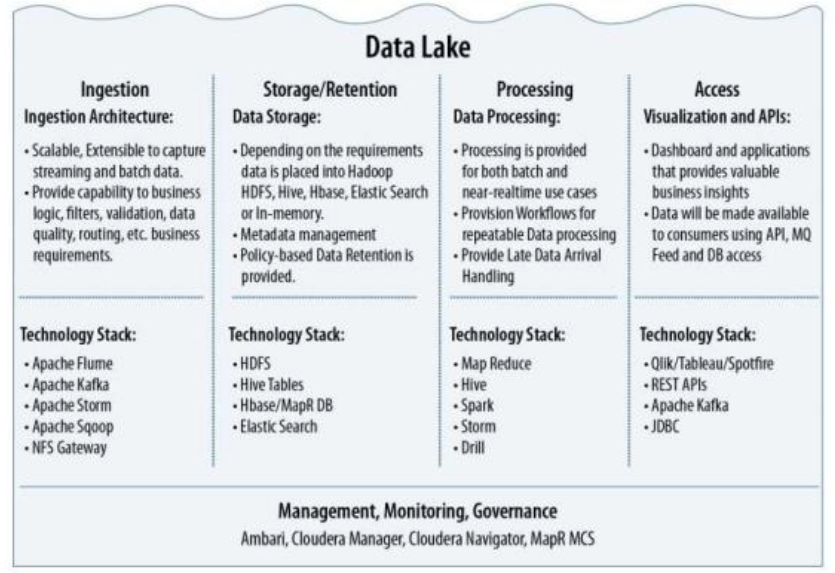
\includegraphics[scale=0.70]{IMAGE10.png}\\
Schema riassuntivo Data Lake
\end{center}
Le componenti di un’architettura data lake sono le seguenti:
\begin{itemize}[noitemsep]
\item Storage, basata su un’architettura HDFS.
\item Data Ingestion, ovvero l’acquisizione di dati da fonti esterne che avviene tramite sistemi come Sqoop (RDBMS), Flume (Web Servers), Kafka o Storm (Streaming Data).
\item Data Processing, che si suddivide in tre fasi: data
preparation, data analystics e result provisioning for consumption. Per effettuare tutte queste operazioni ci si serve di software quali MapReduce, Spark, Flink o Storm. Per eseguire molte attività di manipolazione viene spesso utilizzato NiFi, ovvero un tool workflow based che integra vari applicativi.
\item Data Governance, che comprende Lineage, Integration, Authentication and Authorization, Search, Quality, Audit Logging, Metadata Management, Lifecycle Management e Security.
\end{itemize}
Per acquisire dati in real-time è necessario catturare ogni aspetto di tali dati e con il minimo ritardo possibile. Inoltre, talvolta è necessario sia immagazzinare questi dati in streaming che analizzarli all’istante. La principale limitazione dell’architettura Lambda è che per fare ciò, la logica architetturale va implementata due volte, spesso con tool diversi (Storm, Flink, Spark, …). L’architettura Kappa risolve questo problema.
\section{Data quality and integration}
Fasi molto importanti nell'analisi dei dati sono: la “verifica della qualità dei dati” (Data Understanding), di “pulizia” e di “integrazione” dei dati (Data Preparation).\newline Come primo aspetto, bisogna concentrarsi sui casi di “deduplication”; in altre parole bisogna chiedersi: ci sono record nella stessa tabella che si riferiscono allo stesso oggetto/persona della realtà? Si possono stabilire molteplici regole per decidere se due record si riferiscono allo stesso oggetto, sia sintattiche che semantiche. Una volta individuati due record “analoghi”, bisogna unirli (data fusion) in un solo record contenente le informazioni “corrette”. Una volta analizzato questo aspetto di “qualità” dei dati, immaginiamoci di dover integrare una tabella con un’altra e quindi di dover cercare i record delle due tabelle diverse che sono collegati tra loro. Questo processo si chiama “record linkage” e può essere svolto, ad esempio, individuando le chiavi delle due tabelle (una primaria e una esterna, ad esempio), e se queste corrispondono si procede con il “merge” dei due record.\newline Tuttavia, se la data quality non è delle migliori (a causa di input sbagliati o di standard non condivisi), di conseguenza anche la data integration sarà scarsa.\newline
La data integration si articola in due fasi: \textbf{record linkage} (identificazione dei set di record che identificano lo stesso “oggetto reale”) e \textbf{data fusion} (scelta di un record unico rappresentativo del set precedente).
\subsection{Record Linkage}
Esistono vari sinonimi per questa fase: Object Identification, Deduplication (su un dataset), Object Matching e molti altri. L’output di un algoritmo di record linkage può essere: “matching tuples”, “not matching” o “don’t know” (o “possible matching").\newline
Esistono più tecniche di record linkage:
\begin{itemize}[noitemsep]
\item Empirica, ovvero due tuple vengono unite se la loro distanza (in termini sintattici o anche altre forme di distanza) è piccola.
\item Probabilistica, ovvero una generalizzazione sulla popolazione di regole estratte da un campione.
\item Knowledge Based, ovvero decisioni prese seguendo regole prestabilite.
\item Mixed, ovvero un misto tra il secondo e il terzo approccio.
\end{itemize}
Il record linkage può essere effettuato anche tra set di dati in formati diversi.
%Da valutare se è il caso di aggiungere anche la parte dedicata all'approccio probabilistico.
\subsection{Data Fusion}
Durante questa fase si possono incontrare possibili conflitti.\newline 
Esistono perciò delle strategie per gestire tali conflitti:
\begin{itemize}[noitemsep]
\item Conflict Ignoring, che ignora il problema lasciando la risoluzione all’utente.
\item Conflict Avoiding, che gestisce il problema generalmente scegliendo una delle fonti come “la più affidabile” e creando il record rappresentativo da quella fonte.
\item Conflict Resolution, che fa attenzione a dati e metadati prima di decidere sulla risoluzione del conflitto. Questa strategia può essere divisa in “deciding” (quando viene scelto un valore tra quelli esistenti) e “mediating” (quando viene scelto un valore che non appartiene per forza a quelli esistenti, per esempio la media).
\end{itemize}
\pagebreak
\printbibliography
\end{document}
